\section{Вычислительные эксперименты}
Обозначения, которые используются далее: \\
all\_speakers = [speaker1, speaker2, speaker3, speaker4, speaker5, speaker6] \\
all\_male\_speakers = [speaker1, speaker2, speaker3, speaker4, speaker5]
\subsection{Описание экспериментов}
Для каждого из двух типов нейронных сетей, многослойного персептрона и свёрточной сети, проводится три эксперимента:
\begin{enumerate}[leftmargin=2cm]
	\item нейронная сеть обучается на первом дикторе с мужским голосом, тестирование производится на каждом дикторе
	\item нейронная сеть обучается на всех дикторах с мужским голосом, тестирование производится на каждом дикторе
	\item нейронная сеть обучается на всех дикторах, тестирование производится на каждом дикторе.
\end{enumerate}

Обучение производится со следующими параметрами:
\begin{itemize}[leftmargin=2cm]
	\item после каждой эпохи тренировочные данные перемешиваются
	\item 15\% тренировочных данных в каждой эпохе - валидационные
	\item метрика для оценки эффективности - точность (в библиотеке Keras называется accuracy)
	\item функция потерь - категориальная кросс-энтропия (categorical\_crossentropy)
	\item алгоритм оптимизации - Adam
	\item количество эпох обучения сети - 50
	\item ранняя остановка обучения сети, если в течение 20 эпох значение функции потерь на валидационных данных не улучшается.
\end{itemize}

В случае обучения на all\_speakers, помимо тестирования строится матрица путаницы (confusion matrix) для каждого из четырёх пороговых значений: 0.5, 0.6, 0.7, 0.8. Анализируя её, можно подобрать оптимальное пороговое значение для более удобного использования интерфейса распознавания речевых команд уже при его внедрении в программное обеспечение медиаплеера. 

Смысл порогового значения следующий.
\begin{itemize}[leftmargin=2cm]
	\item Если максимальный элемент в выходном тензоре нейронной сети ниже порогового значения, то команда распознаётся как тишина. В этом случае интерфейс медиаплеера просит повторить команду ещё раз. 
	\item Если максимальный элемент в выходном тензоре нейронной сети выше или равен пороговому значению, то команда распознаётся как соответствующая индексу этого максимального элемента. 
\end{itemize}
\subsection{Результаты экспериментов}
Графики обучения многослойного персептрона приведены на рисунках \ref{fig:mlp_speaker1_train_graphs}, \ref{fig:mlp_all_male_speakers_train_graphs}, \ref{fig:mlp_all_speakers_train_graphs}.

\begin{figure}[H]
	\[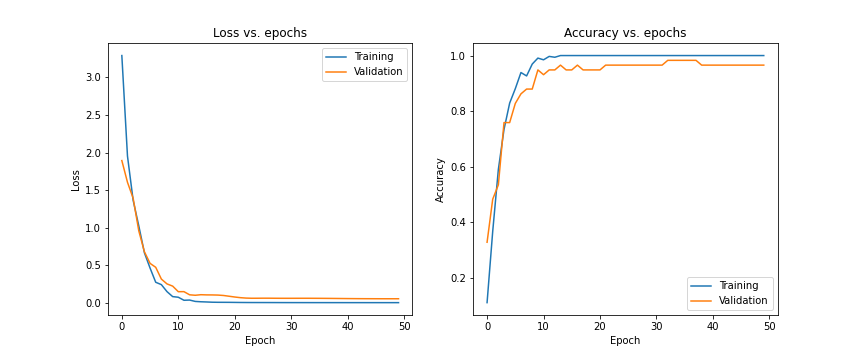
\includegraphics[scale=0.4]{mlp_speaker1_train_graphs.png}\]
	\caption{Графики функций потерь и точности многослойного персептрона в течение обучения на speaker1}
	\label{fig:mlp_speaker1_train_graphs}
\end{figure}

\begin{figure}[H]
	\[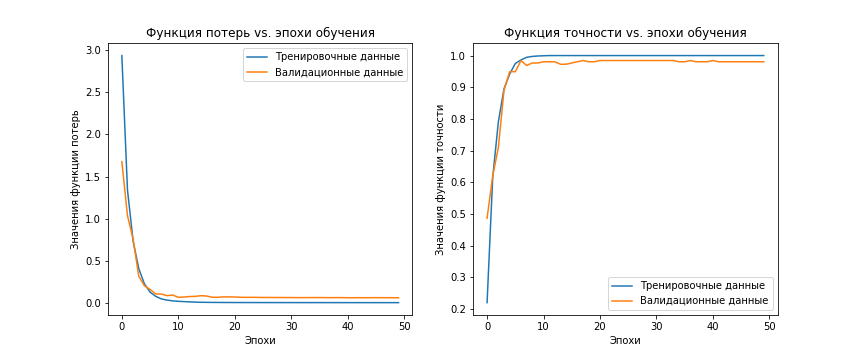
\includegraphics[scale=0.4]{mlp_all_male_speakers_train_graphs.png}\]
	\caption{Графики функций потерь и точности многослойного персептрона в течение обучения на all\_male\_speakers}
	\label{fig:mlp_all_male_speakers_train_graphs}
\end{figure}

\begin{figure}[H]
	\[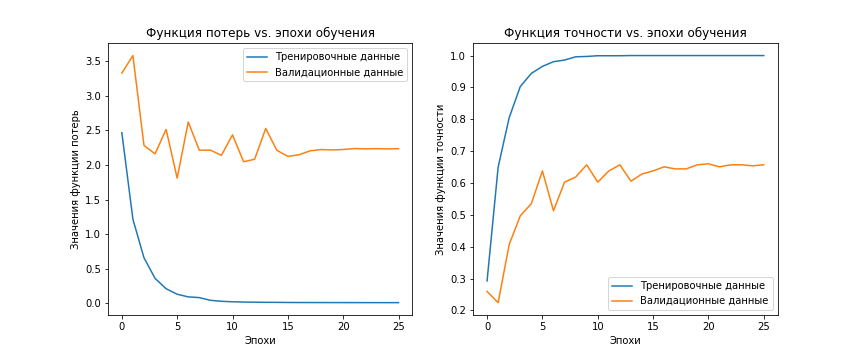
\includegraphics[scale=0.4]{mlp_all_speakers_train_graphs.png}\]
	\caption{Графики функций потерь и точности многослойного персептрона в течение обучения на all\_speakers}
	\label{fig:mlp_all_speakers_train_graphs}
\end{figure}


Графики обучения свёрточной сети приведены на рисунках \ref{fig:cnn_speaker1_train_graphs}, \ref{fig:cnn_all_male_speakers_train_graphs}, \ref{fig:cnn_all_speakers_train_graphs}.

\begin{figure}[H]
	\[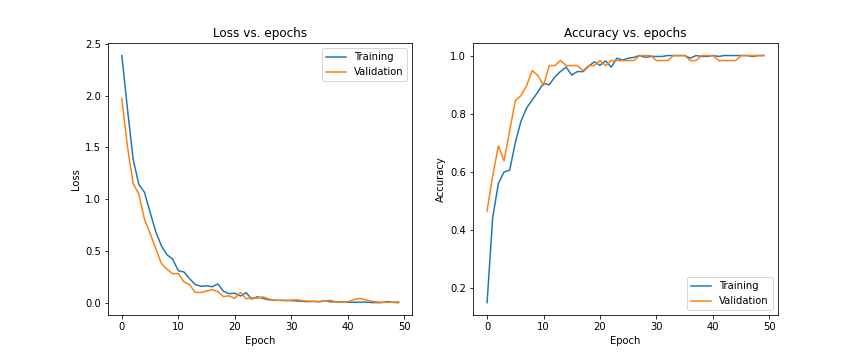
\includegraphics[scale=0.4]{cnn_speaker1_train_graphs.png}\]
	\caption{Графики функций потерь и точности свёрточной сети в течение обучения на speaker1}
	\label{fig:cnn_speaker1_train_graphs}
\end{figure}

\begin{figure}[H]
	\[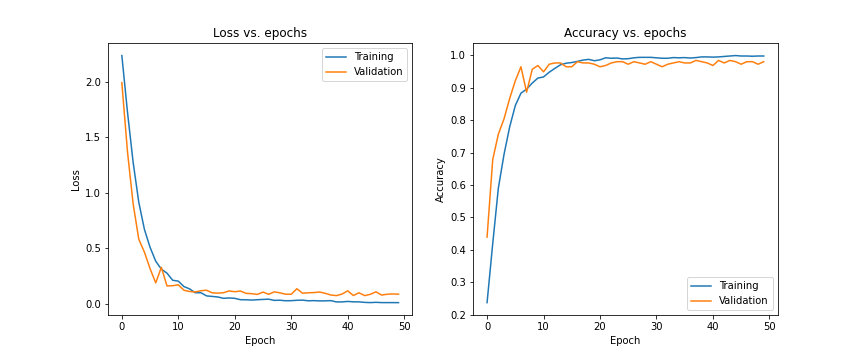
\includegraphics[scale=0.4]{cnn_all_male_speakers_train_graphs.png}\]
	\caption{Графики функций потерь и точности свёрточной сети в течение обучения на all\_male\_speakers}
	\label{fig:cnn_all_male_speakers_train_graphs}
\end{figure}

\begin{figure}[H]
	\[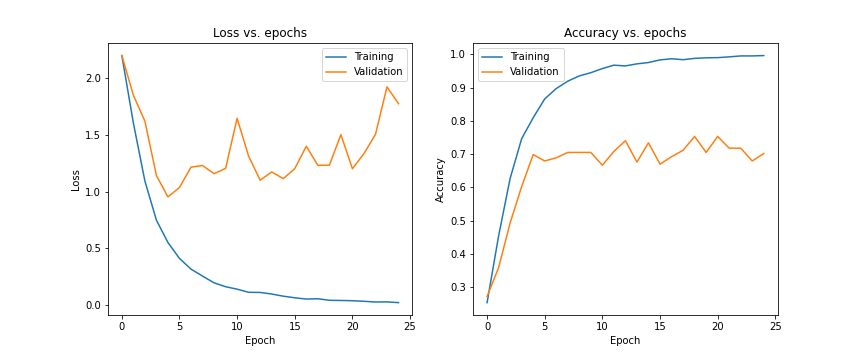
\includegraphics[scale=0.4]{cnn_all_speakers_train_graphs.png}\]
	\caption{Графики функций потерь и точности свёрточной сети в течение обучения на all\_speakers}
	\label{fig:cnn_all_speakers_train_graphs}
\end{figure}

Матрицы путаницы для многослойного персептрона при обучении на all\_speakers представлены на рисунке \ref{fig:mlp_cm_all_speakers}.

\begin{figure}[H]
	\[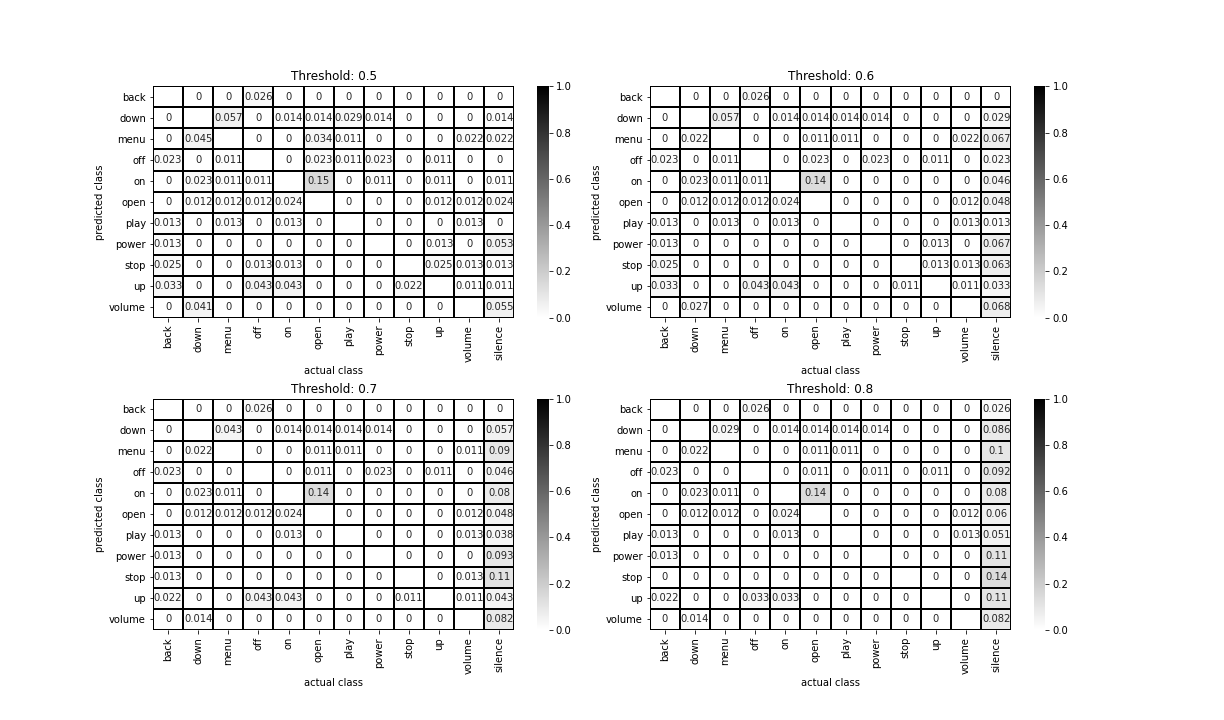
\includegraphics[scale=0.4]{mlp_cm_all_speakers.png}\]
	\caption{Матрицы путаниц для многослойного персептрона при обучении на all\_speakers}
	\label{fig:mlp_cm_all_speakers}
\end{figure}


Матрицы путаницы для свёрточной сети при обучении на all\_speakers представлены на рисунке \ref{fig:cnn_cm_all_speakers}.

\begin{figure}[H]
	\[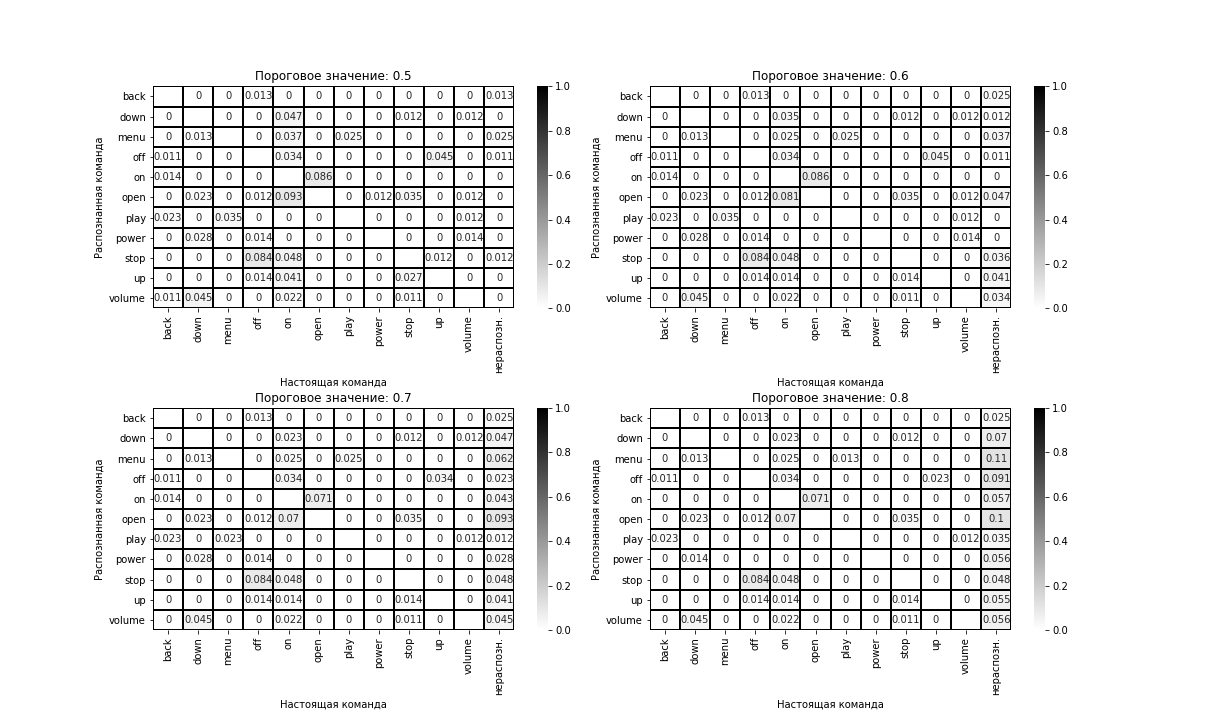
\includegraphics[scale=0.4]{cnn_cm_all_speakers.png}\]
	\caption{Матрицы путаницы для свёрточной сети при обучении на all\_speakers}
	\label{fig:cnn_cm_all_speakers}
\end{figure}

Результаты тестирования представлены в таблице \ref{table:test_summary}. 

\begin{table}[H]
\small
\centering
\csvautotabular[respect underscore=true]{csv/test_summary.csv}
\caption{Результаты вычислений}
\label{table:test_summary}
\end{table}